%%%%%%%%%%%%%%%%%%%%%%%%%%%%%%%%%%%%%%%%%%%%%%%%%%%%%%%%%%%%%%%%%%%%%%%%%%%%%
%
%  System        : 
%  Module        : 
%  Object Name   : $RCSfile$
%  Revision      : $Revision$
%  Date          : $Date$
%  Author        : $Author$
%  Created By    : Robert Heller
%  Created       : Sat Jul 15 10:35:16 2017
%  Last Modified : <170730.1748>
%
%  Description 
%
%  Notes
%
%  History
% 
%%%%%%%%%%%%%%%%%%%%%%%%%%%%%%%%%%%%%%%%%%%%%%%%%%%%%%%%%%%%%%%%%%%%%%%%%%%%%
%
%    Copyright (C) 2017  Robert Heller D/B/A Deepwoods Software
%			51 Locke Hill Road
%			Wendell, MA 01379-9728
%
%    This program is free software; you can redistribute it and/or modify
%    it under the terms of the GNU General Public License as published by
%    the Free Software Foundation; either version 2 of the License, or
%    (at your option) any later version.
%
%    This program is distributed in the hope that it will be useful,
%    but WITHOUT ANY WARRANTY; without even the implied warranty of
%    MERCHANTABILITY or FITNESS FOR A PARTICULAR PURPOSE.  See the
%    GNU General Public License for more details.
%
%    You should have received a copy of the GNU General Public License
%    along with this program; if not, write to the Free Software
%    Foundation, Inc., 675 Mass Ave, Cambridge, MA 02139, USA.
%
% 
%
%%%%%%%%%%%%%%%%%%%%%%%%%%%%%%%%%%%%%%%%%%%%%%%%%%%%%%%%%%%%%%%%%%%%%%%%%%%%%

% $Header: /cvsroot/latex-beamer/latex-beamer/solutions/conference-talks/conference-ornate-20min.en.tex,v 1.6 2004/10/07 20:53:08 tantau Exp $

%\documentclass[ignorenonframetext]{beamer}
%\documentclass[letterpaper]{article} \usepackage{beamerarticle}

% This file is a solution template for:

% - Talk at a conference/colloquium.
% - Talk length is about 20min.
% - Style is ornate.



% Copyright 2004 by Till Tantau <tantau@users.sourceforge.net>.
%
% In principle, this file can be redistributed and/or modified under
% the terms of the GNU Public License, version 2.
%
% However, this file is supposed to be a template to be modified
% for your own needs. For this reason, if you use this file as a
% template and not specifically distribute it as part of a another
% package/program, I grant the extra permission to freely copy and
% modify this file as you see fit and even to delete this copyright
% notice. 


\mode<presentation>
{
  \usetheme{Warsaw}
  \pgfdeclareimage[height=0.5cm]{deepwoods-software}{largeHeader}
  \logo{\pgfuseimage{deepwoods-software}}
  
  % or ...
}

\mode<article>{
  \usepackage{fullpage}
}

\usepackage[english]{babel}
% or whatever

\usepackage[latin1]{inputenc}
% or whatever

\usepackage{times}
\usepackage[T1]{fontenc}
% Or whatever. Note that the encoding and the font should match. If T1
% does not look nice, try deleting the line with the fontenc.
\usepackage{graphicx}

\title{Raspberry Pi Junction}

%\subtitle
%{Include Only If Paper Has a Subtitle}

\author{Robert Heller \\ \texttt{heller@deepsoft.com}}

\institute{Deepwoods Software}

\date{Summer, 2017}

%\subject{LCC CTC Panels}
% This is only inserted into the PDF information catalog. Can be left
% out. 



% If you have a file called "university-logo-filename.xxx", where xxx
% is a graphic format that can be processed by latex or pdflatex,
% resp., then you can add a logo as follows:

% \pgfdeclareimage[height=0.5cm]{university-logo}{university-logo-filename}
% \logo{\pgfuseimage{university-logo}}


% Delete this, if you do not want the table of contents to pop up at
% the beginning of each subsection:
%\AtBeginSubsection[]
%{
%  \begin{frame}<beamer>
%    \frametitle{Outline}
%    \tableofcontents[pausesections]
%  \end{frame}
%}


% If you wish to uncover everything in a step-wise fashion, uncomment
% the following command: 

%\beamerdefaultoverlayspecification{<+->}


\begin{document}

\begin{frame}
  \titlepage
\end{frame}

%\begin{frame}
%  \frametitle{Outline}
%  \tableofcontents
%  % You might wish to add the option [pausesections]
%\end{frame}

% Structuring a talk is a difficult task and the following structure
% may not be suitable. Here are some rules that apply for this
% solution: 

% - Exactly two or three sections (other than the summary).
% - At *most* three subsections per section.
% - Talk about 30s to 2min per frame. So there should be between about
%   15 and 30 frames, all told.

% - A conference audience is likely to know very little of what you
%   are going to talk about. So *simplify*!
% - In a 20min talk, getting the main ideas across is hard
%   enough. Leave out details, even if it means being less precise than
%   you think necessary.
% - If you omit details that are vital to the proof/implementation,
%   just say so once. Everybody will be happy with that.

\section{What it is}

This is Raspberry Pi Junction, a simple interlocking off the main line at Mile 
Post 314 that goes past the Mad Hatter Pie Shop.

The junction itself and the adjacent blocks are controlled by a Raspberry Pi 
Model 3 B+ (sirtopemhat), which has five HAT (Hardware Attached on Top) boards.

The HAT boards interface to the layout control elements on the layout. The
layout control elements include one Circuitron Tortoise stall-motor switch
machine, a Circuits4Tracks Quad Occupancy Detector, and six color light
signals.  Also the lighting of the Mad Hatter Pie Shop can be controlled by 
the Raspberry Pi.

\begin{frame}
   \frametitle{What it is}
   \begin{itemize}
   \item Raspberry Pi Junction is a simple spur off the main line at Mile Post 
   314 that goes past the Mad Hatter Pie Shop. 
   \item It and the adjacent blocks are controlled by a Raspberry Pi Model 3 
   B+ (sirtopemhat), which has five HAT (Hardware Attached on Top) boards.
   \item The HAT boards interface to the layout control elements on the 
   layout.
   \end{itemize}
\end{frame} 

\section{The basic layout}

\begin{frame}
   \frametitle{The basic layout}
   \includegraphics[width=3.5in]{PiJunction.png}
\end{frame}

\section{The HATs}

Each of the HATs provide the hardware to interface the Pi to the control
elements on the layout. This is done using the GPIO pins on the Pi's 40-pin
GPIO header.  

\begin{frame}
   \frametitle{The HAT boards}
   \begin{description}
   \item[RTC Hat] This is just a DS1307 Real Time Clock module, used to keep 
   time when the Pi is shutdown.
   \item[SMCSenseHAT] This HAT controls the Circuitron Tortoise stall-motor 
   switch machine and sense its position.
   \item[QuadSSSQuadIn] This HAT provides the inputs for the Circuits4Tracks 
   Quad Occupancy Detector and also controls the structure light for the Mad 
   Hatter Pie Shop.
   \item[MCP23017Hat] There are two of these boards and they control the 
   lighting of the signals.
   \end{description}
\end{frame}

\subsection{SMCSenseHAT}

The SMCSenseHAT board uses GPIO pins to control and sense two Circuitron
Tortoise (or similar) stall-motor switch machines. Two GPIO pins drive the
stall-motors (one for each stall-motor) and two GPIO pins return the point
state for the stall-motors (one for each stall-motor). The OpenLCB\_PiGPIO
program implements a LCC/OpenLCB node that interfaces this HAT to the
LCC/OpenLCB network, consuming events to activate the stall-motor(s), and
produce events to indicate the point position.

\begin{frame}
    \frametitle{The SMCSenseHAT board}
    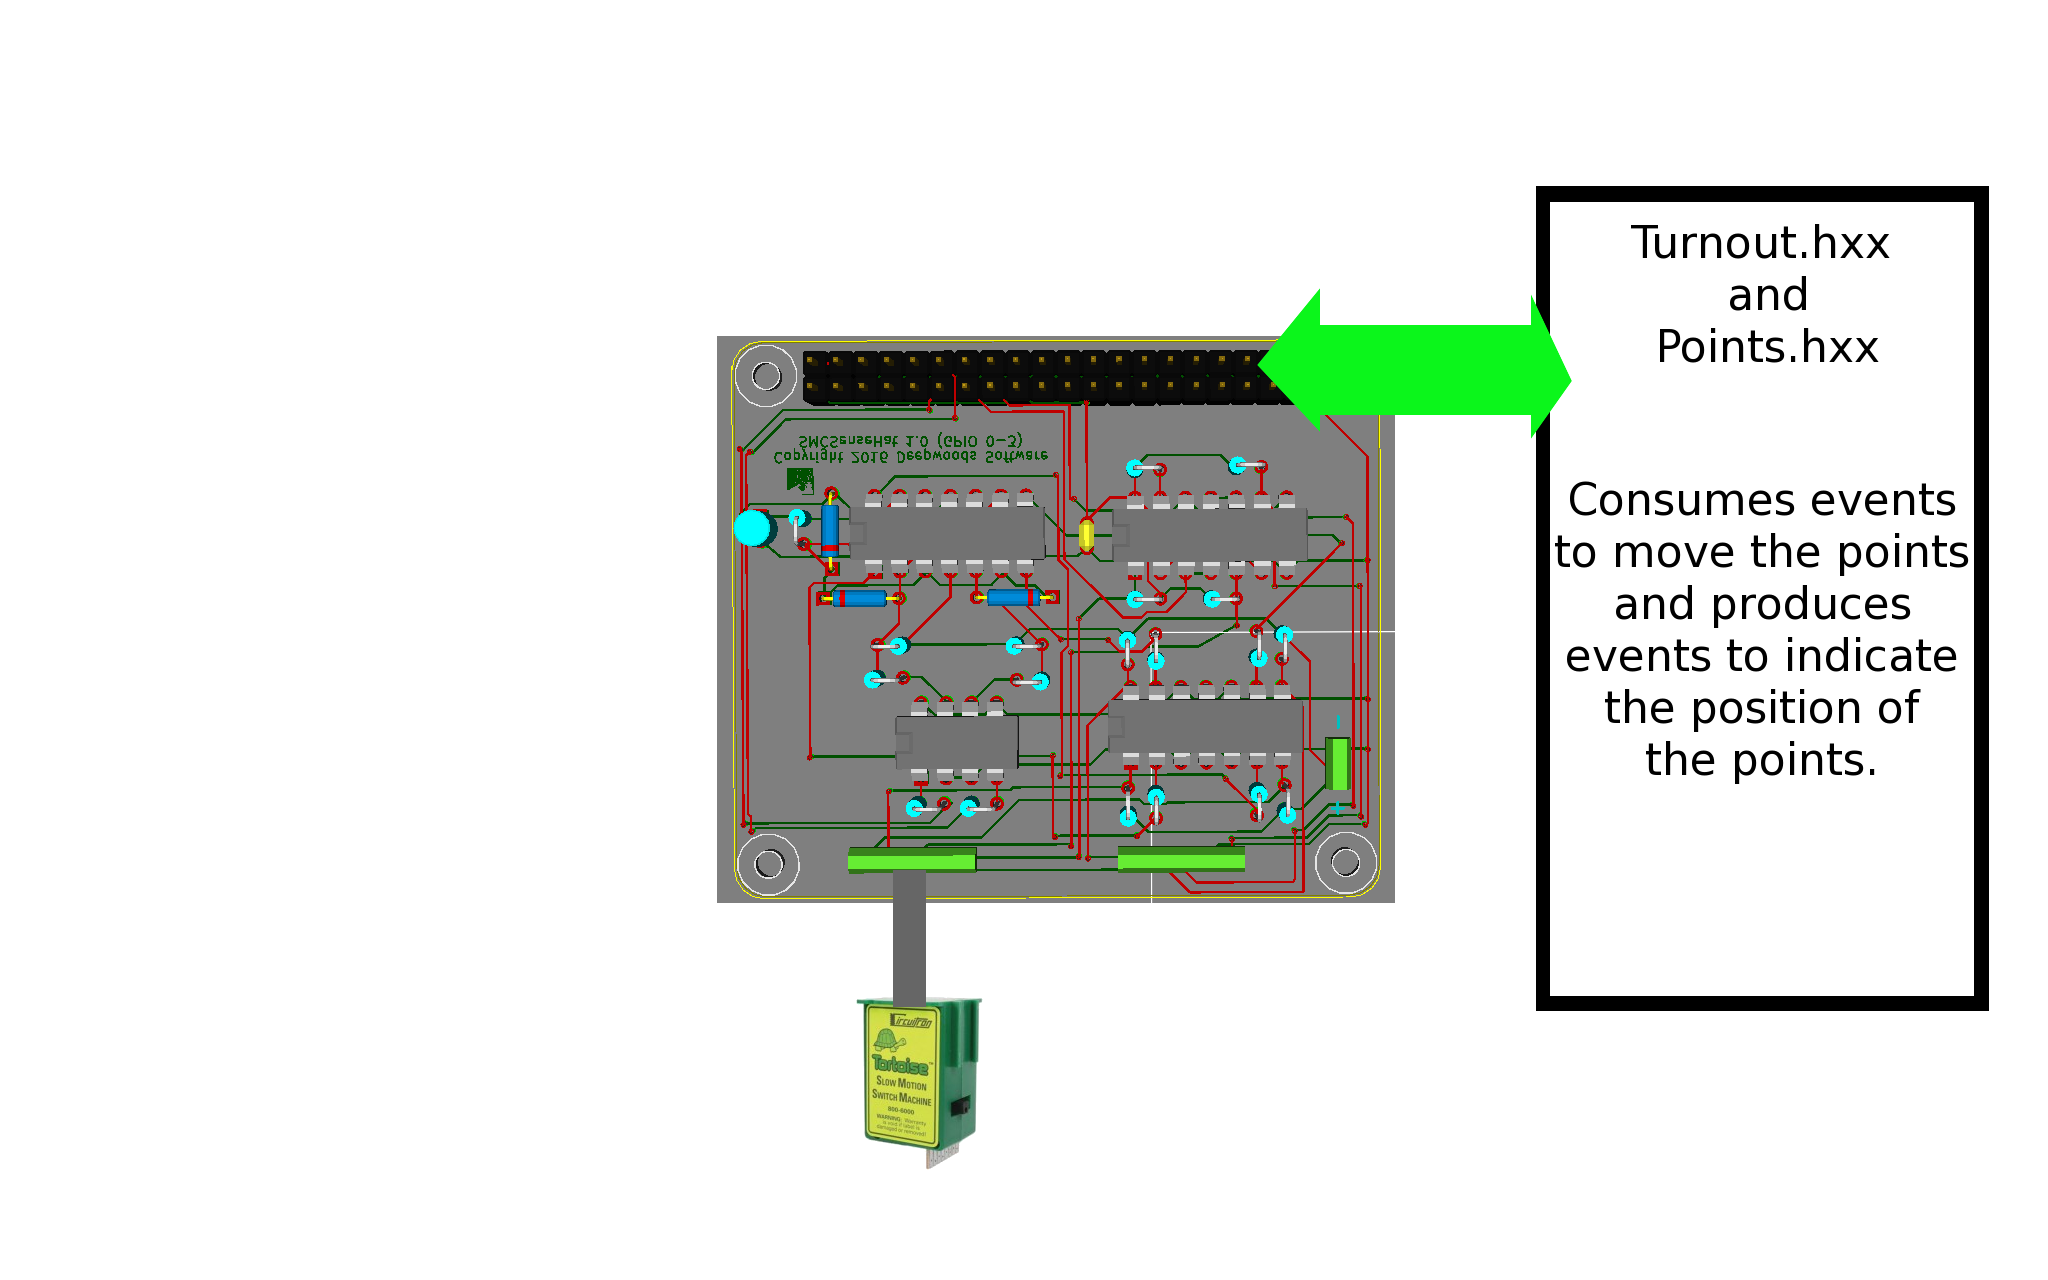
\includegraphics[width=3.5in]{SMCSenseHAT-frame.png}
\end{frame}

\subsection{QuadSSSQuadIn}

The QuadSSSQuadIn uses a MCP23008 I2C I/O expander chip to implement four 5V 
Logic inputs and four SSR (Solid State Relay) outputs.  The four inputs are 
connected to the Circuits4Tracks Quad Occupancy Detector's outputs and one of 
the SSR outputs controls the lighting of the Mad Hatter Pie Shop.  The 
OpenLCB\_PiMCP23008 program implements a LCC/OpenLCB node that interfaces this 
HAT to the LCC/OpenLCB network, producing events for block occupancy and 
consuming events to turn the Mad Hatter Pie Shop's light on and off.

\begin{frame}
    \frametitle{The QuadSSSQuadIn board}
    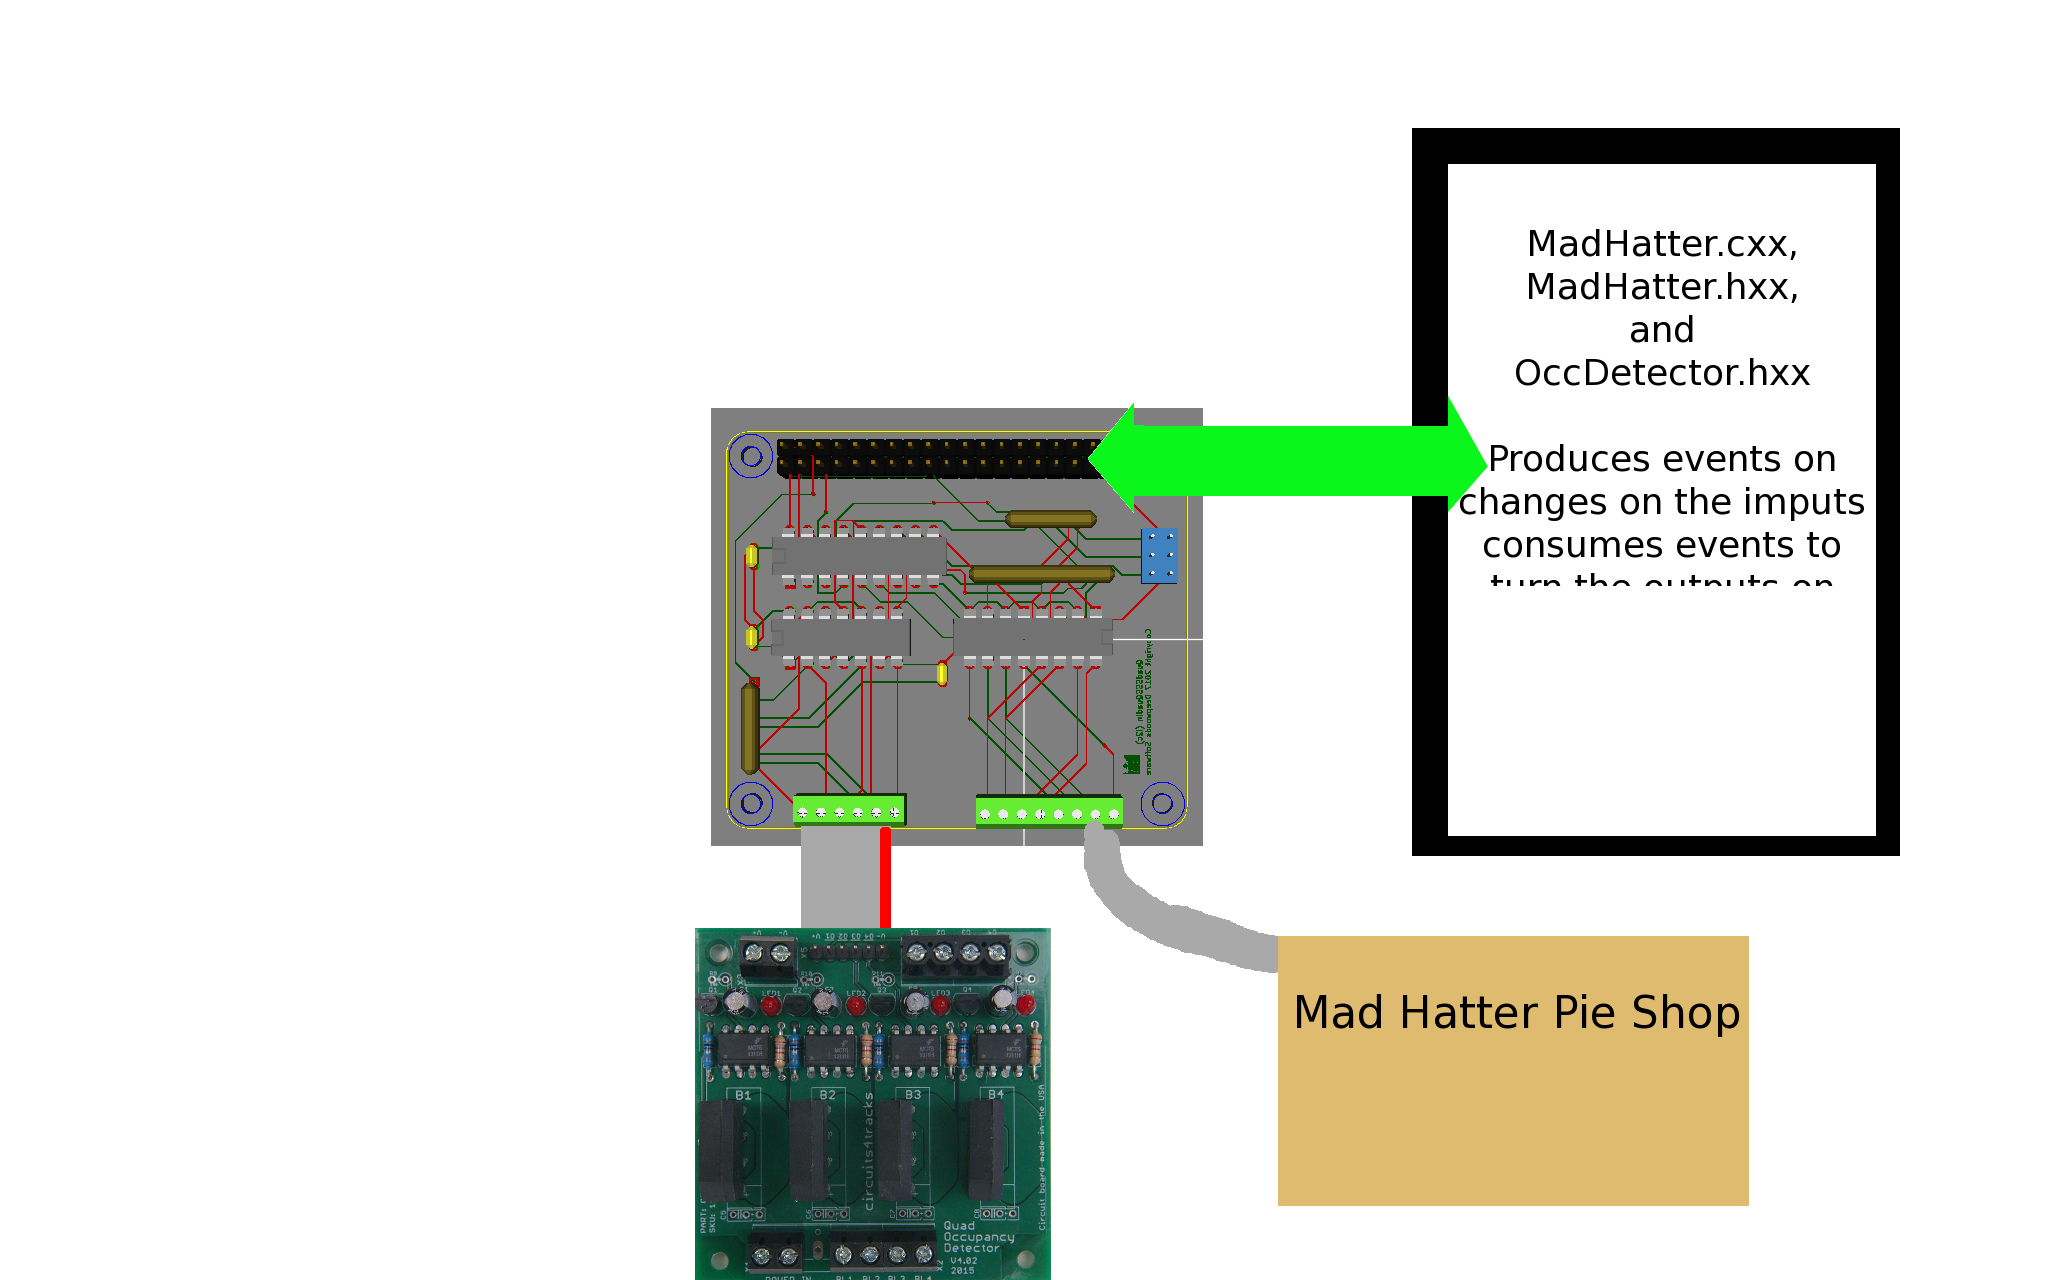
\includegraphics[width=3.5in]{QuadSSSQuadIn-frame.png}
\end{frame}


\subsection{MCP23017Hat}

The MCP23017Hat uses a MCP23017 I2C I/O expander chip to implement 16 3.3V 
GPIO pins, in two banks of 8.  There are two of these HATs and they are used 
to drive the 22 LEDs in the 6 signals.  There are three octal (8) LED driver 
boards to actually drive the LEDs.  There are two processes running the 
OpenLCM\_PiMCP23017\_signal program, creating two LCC nodes to handle all of 
the signals.

\begin{frame}
   \frametitle{The MCP23017Hat board}
   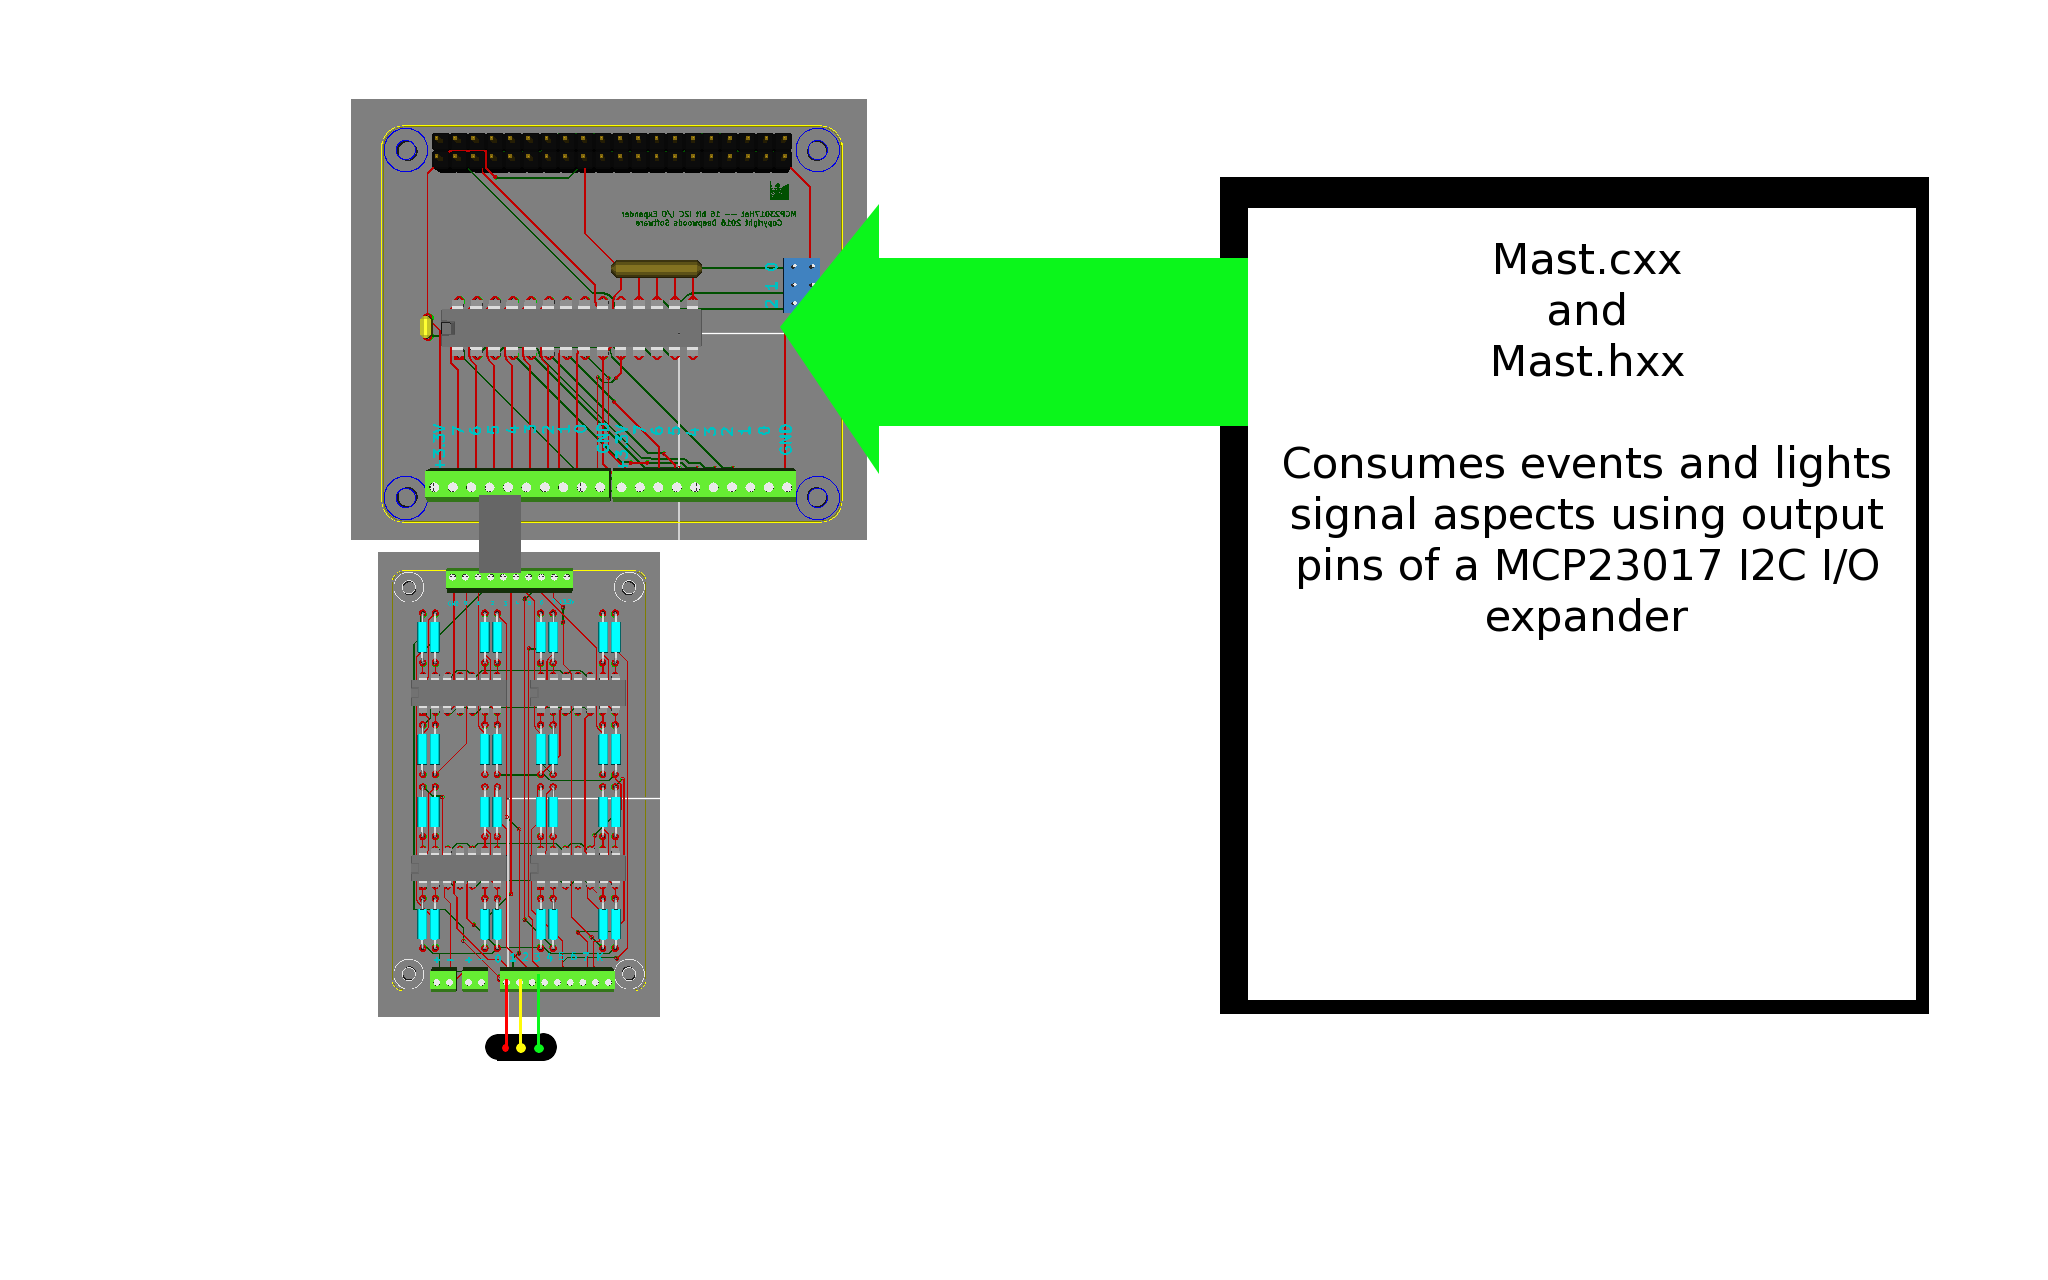
\includegraphics[width=3.5in]{MCP23017Hat-frame.png}
\end{frame}

\section{The LCC/OpenLCB network}

On the software side, the Raspberry Pi implements a ``virtual'' LCC/OpenLCB
``network''. The Model Railroad System from Deepwoods Software includes daemon
programs that interface to the HATs and to provide a virtual network for them
to communicate over. This includes a Tcp/Ip ``hub'' daemon, and a set of
OpenLCB ``node'' daemons, along with a program, Dispatcher, that can be used
to to create a CTC (Dispatcher) panel program. Each of the node daemons
interfaces to one HAT, plus a pair of additional node daemons, one to
implement the ``logic'' of the layout and one to implement a CTC (Dispatcher)
panel. All of the nodes communite with each other through the ``hub'' daemon
by passing LCC Event Report messages to each other. 

\begin{frame}
    \frametitle{The LCC/OpenLCB network}
    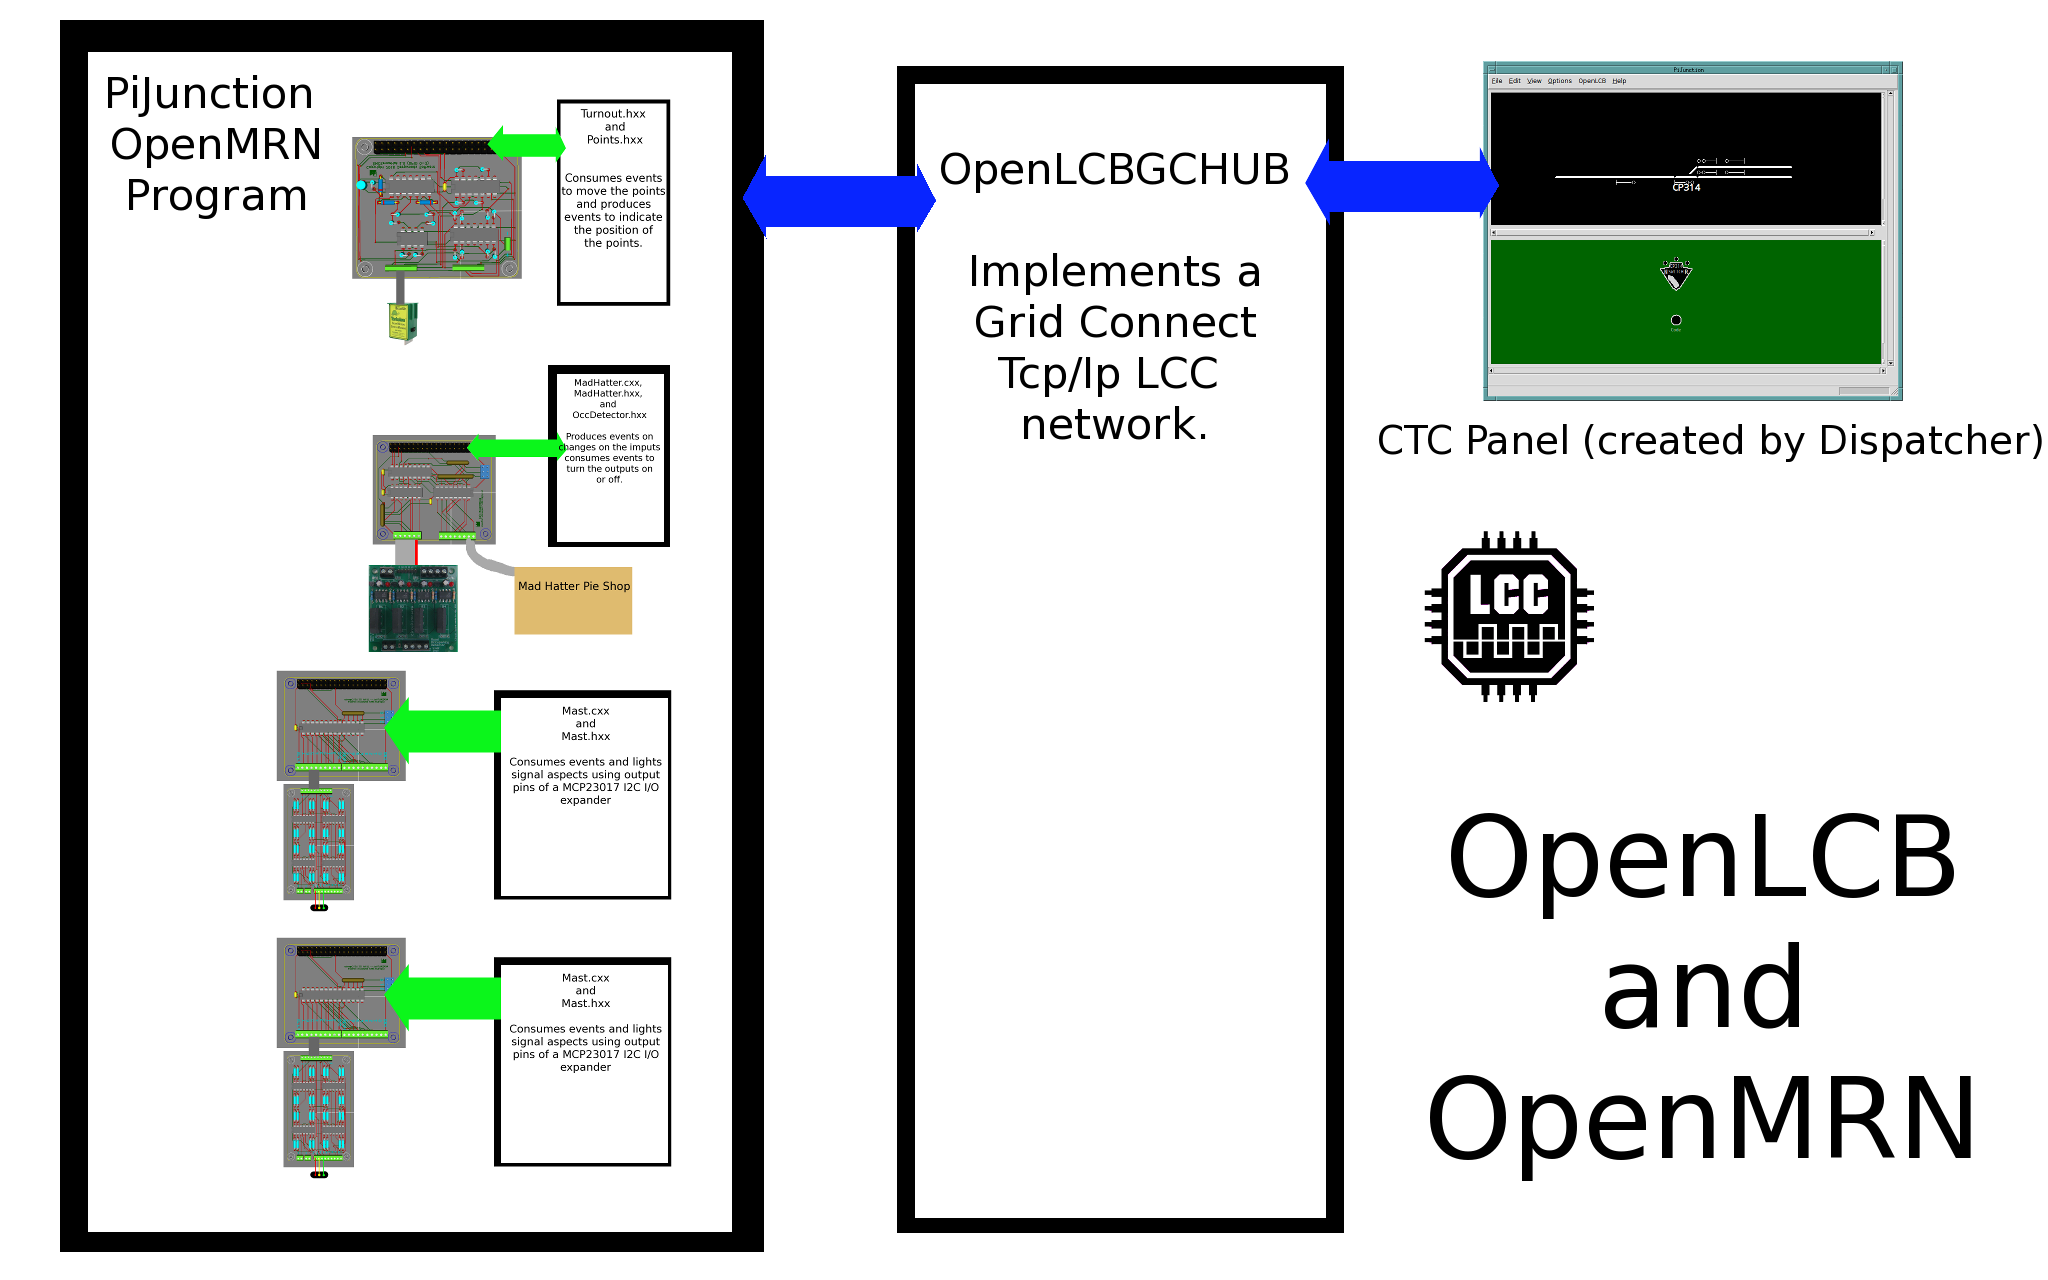
\includegraphics[width=3.5in]{LCC-Network-frame.png}
\end{frame}


\section{Traction control -- Driving the loco}

The locomotive is powered by DCC using a Lenz command station / booster.  I 
use a Pi Engineering Rail Driver in place of a DCC throtle.

The Rail Driver is a USB HID device and I use the Model Railrail System 
raildriverd daemon to drive it, using the Raildriver Support library and use 
the XPressNet library to talk to the Lenz command station / booster unit.

\begin{frame}
    \frametitle{Traction control}
    \includegraphics[width=3.5in]{Raildriver-DCC-USB-frame.png}
\end{frame}

\end{document}
